%===============================================================================
\begin{frame}
\frametitle{Прототипирование нейронных сетей на FPGA}
\begin{columns}[T]
    \column{0.6\textwidth}

    \begin{itemize}
        \item Ставилась задача реализации на ПЛИС нейронной сети для распознавания изображений (рукописных цифр из базы MNIST)
        \item Простая однослойная нейронная сеть (7850 параметров) позволяет достичь относительно невысокой точности 92,5\%
        \item При добавлении скрытых слоев число параметров сети стремительно увеличивается
    \end{itemize}

    \column{0.4\textwidth}
    \begin{block}{\centering}
        \vspace{1mm}
        \centering
        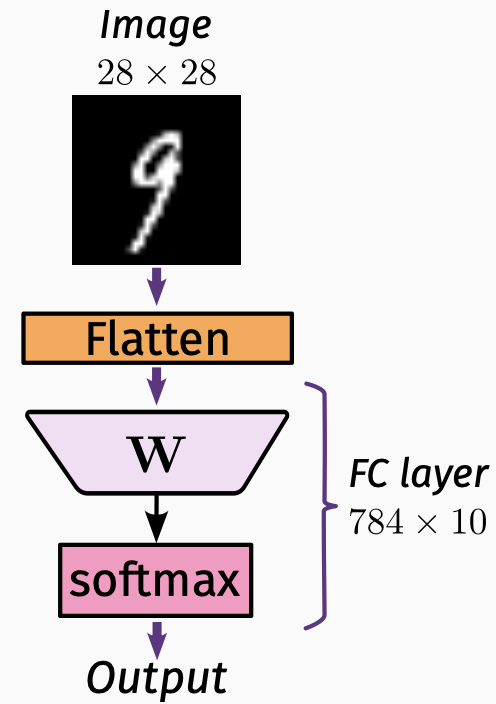
\includegraphics[width = 0.7\textwidth]{pics/simple_nn.png} 
        % \includesvg[height = 0.5\textheight]{RGB_multidim_data.svg}        
    \end{block}
\end{columns}
\end{frame}
%===============================================================================

\begin{frame}
\frametitle{Особенности существующих реализаций НС на ПЛИС}

\begin{table}[htbp]
    \centering
    \renewcommand{\arraystretch}{1}
    \begin{tabular}{|>{\raggedright\arraybackslash}p{4.5cm}|>{\centering\arraybackslash}p{4.5cm}|>{\centering\arraybackslash}p{3cm}|>{\centering\arraybackslash}p{1.5cm}|}
    \hline
    \textbf{Автор} & \textbf{Архитектура НС} & \textbf{\# Число параметров} & \textbf{Точность} \\
    \hline
    Liang, et al. (2018) & 784-2048-2048-2048-10 & 10 100 000 & 98.32\% \\
    Umuroglu, et al. (2017) & 784-1024-1024-10 & 1 863 690 & 98.40\% \\
    Medus, et al. (2019) & 784-600-600-10 & 891 610 & 98.63\% \\
    Huynh\textsuperscript{1} & 784-126-126-10 & 115 920 & 98.16\% \\
    Huynh\textsuperscript{1} & 784-40-40-40-10 & 34 960 & 97.20\% \\
    Westby, et al.\textsuperscript{2} & 784-12-10 & 9 550 & 93.25\% \\
    \hline
\end{tabular}
\end{table}
    
    \vspace{0.5em}
    
    \noindent\textsuperscript{1}T. V. Huynh, “Deep neural network accelerator based on FPGA,” in 4th NAFOSTED Conference on Information and Computer Science, 2017, pp. 254--257.\\
    \textsuperscript{2}I. Westby, et al. “FPGA acceleration on a multilayer perceptron neural network for digit recognition,” \textit{Journal of Supercomputing}, 2021, vol. 77, no. 12, pp. 356--373.
    
\end{frame}
%===============================================================================